\documentclass[../main.tex]{subfiles}

\graphicspath{{\subfix{../imgs/}}}

\begin{document}

\section{Dataset}
\begin{frame}[t]
    \frametitle{Dataset}

    \begin{block}{Data Description}
        The dataset consists of 155 primary and 155 metastatic 
        melanoma stained regions of interest (ROI) images, scanned at 40x 
        magnification with a resulution of 1024x1024 pixels.
        For the ROIs, annotations of both tissue and 
        nuclei are provided, along with a context ROI 
        of 5120x5120 pixels centered around the ROI.
    \end{block}

\end{frame}

\begin{frame}[t]
    \frametitle{Dataset}

    \begin{block}{Traning Dataset}
        \small
        The traning set consists of:
        \begin{itemize}
            \item 103 primary melanoma \& 103 metastatic melanoma ROI
            \item A total of 97.429 nuclei is spread across the two 
            classes
        \end{itemize}
    \end{block}

    \begin{block}{Preliminary Test Set }
        \small
        The preliminary test set consists of:
        \begin{itemize}
            \item 5 primary melanoma \& 5 metastatic melanoma ROI
            \item A total of 4.860 nuclei is spread across the two 
            classes
        \end{itemize}
    \end{block}

    \begin{block}{Final Test Set}
        \small 
        The final test set consists of:
        \begin{itemize}
            \item 47 primary melanoma \& 47 metastatic melanoma ROI
            \item A total of 45.406 nuclei is spread across the two 
            classes
        \end{itemize}
    \end{block}
\end{frame}

\begin{frame}[c]

    \begin{figure}[h]
        \centering
        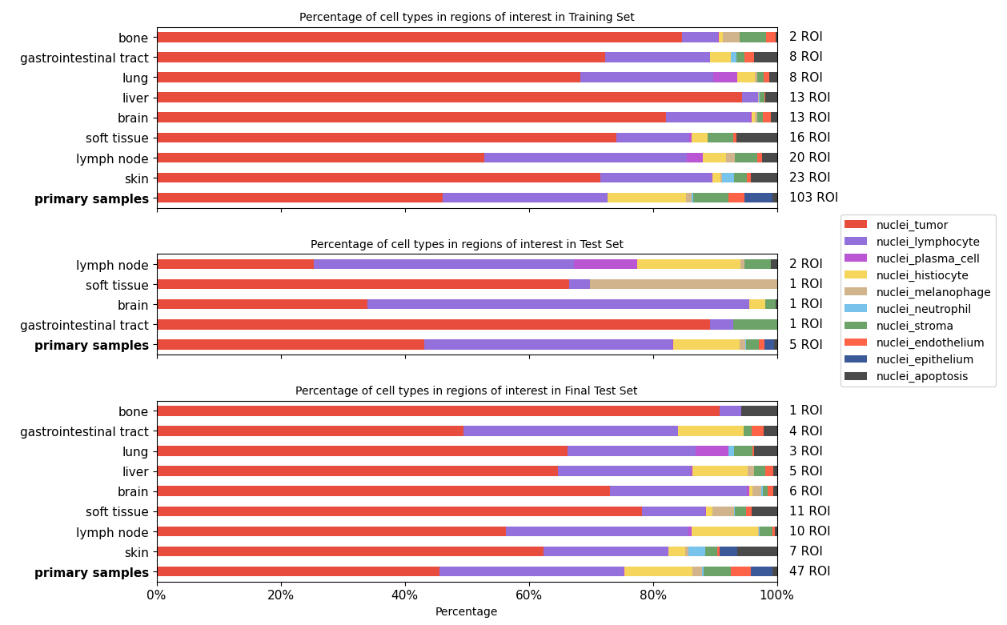
\includegraphics[width=0.95\textwidth]{fig1_nuclei.png}
        \caption{Distribution of nuclei in the datasets.}
    \end{figure}

\end{frame}

\begin{frame}[c]

    \begin{figure}[h]
        \centering
        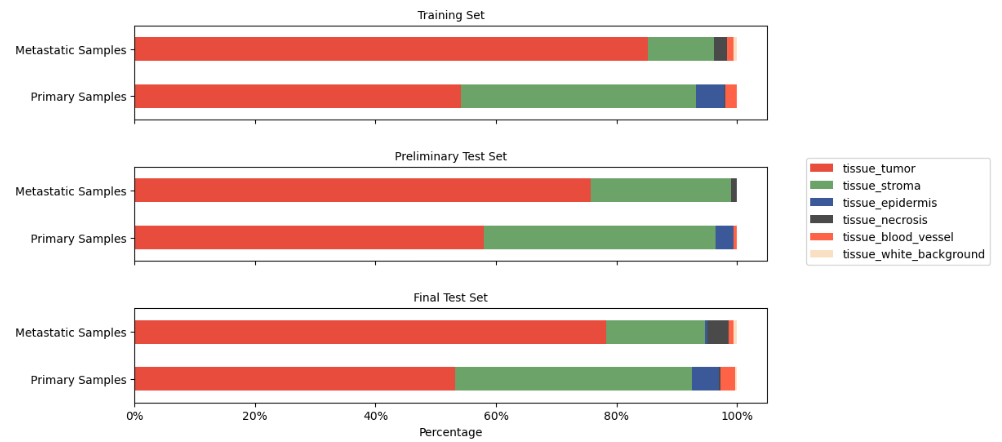
\includegraphics[width=0.95\textwidth]{fig2_nuclei.png}
        \caption{Distribution of tissue class area in the datasets.}
    \end{figure}

\end{frame}

\end{document}